\section{切线}

斜率由 Lua 在坐标系单位下计算，因此即使 \tkzname{xstep} 和 \tkzname{ystep} 不同，切线也是正确的。每条切线由两条半线组成：左侧（l）和右侧（r）。它们的长度由 \tkzname{kl} 和 \tkzname{kr} 给出，单位为 $x$ 轴单位：右半线从切点 $(a, f(a))$ 延伸到点 $(a+k_r, f(a)+k_r f'_+(a))$。设置 $kl=0$ 或 $kr=0$ 时，对应的半线不绘制。

若函数在 $a$ 处不可导，两条半线斜率不同；它们分别计算。

\subsection{绘制切线：\tkzcname{tkzFnTangent}}

\begin{NewMacroBox}{tkzFnTangent}{\oarg{选项}\parg{函数名,$a$}}
\begin{tabular}{lll}
 \toprule
 参数             & 示例 & 说明    \\
 \midrule
 \TAline{函数,a}{(f,0)}{$x=0$ 处的切线}
 \bottomrule
\end{tabular}

\begin{tabular}{lll}
\toprule
选项             & 默认值 & 说明                         \\
\midrule
\TOline{draw}{false}{绘制切点}
\TOline{kl}{1}{左半线长度（$x$ 轴单位）}
\TOline{kr}{1}{右半线长度}
\TOline{clip}{true}{直线裁剪到窗口内}
\bottomrule
\end{tabular}

\emph{其他选项为 \TIKZ\ 选项；样式为 \tkzname{tkzfn tangent}，默认为空。要获得 \tkzname{tkz-fct} 中的箭头效果：}

|\tikzset{tkzfn tangent/.style={->,>=latex}}|
\end{NewMacroBox}

\tkzHand 函数无需绘制；只需定义即可。

%<--------------------------------------------------------------------------->
\subsection{\tkzname{xstep} 和 \tkzname{ystep} 不为 1 时的切线}

无需任何计算：直接使用刻度值即可。

\begin{tkzexample}[vbox]
\begin{tikzpicture}[xscale=1.5]
 \tkzFnInit[xmin=0,xmax=800,xstep=100,
            ymin=0,ymax=1800,ystep=400]
 \tkzFnGrid[color=brown,sub,subdx=50,subdy=200](0,0)(800,1800)
 \tkzFnAxes
 \tkzFnDraw[name=f,color=red,samples=100,domain=0:800]
    {(1/90000)*x^3-(1/100)*x^2+(113/36)*x}
 \tkzFnTangent[draw,color=blue,kr=300,kl=450](f,450)
 \tkzFnText[draw,color=black,fill=brown!50,opacity=0.8](300,1200)
 {$f(x)=\dfrac{1}{90000}x^3 -\dfrac{1}{{100}}x^2 +\dfrac{113}{36}x$}
\end{tikzpicture}
\end{tkzexample}

$450$ 处的斜率为 $\tkzFnPrint[4]{diff(f,450)}$；通过 |\tkzFnPrint[4]{diff(f,450)}| 获得。

%<--------------------------------------------------------------------------->
\subsection{选项 \tkzname{kl}、\tkzname{kr} 和 \tkzname{draw}}

\begin{tkzexample}[]
\begin{tikzpicture}[scale=1.5]
  \tikzset{tkzfn tangent/.style={->,>=latex}}
  \tkzFnInit[xmin=-3,xmax=4,ymin=-4,ymax=2]
  \tkzFnGrid  \tkzFnAxes[ticks=false]
  \tkzFnDraw[name=f,domain=-2.15:3.2]{-x*x+2*x}
  \tkzFnDefPoint[draw](f,2){A}
  \tkzFnTangent[kl=0,draw](f,-1)
  \tkzFnTangent[draw](f,1)
  \tkzFnTangent[kr=0,draw](f,3)
  \tkzFnRep
\end{tikzpicture}
\end{tkzexample}

%<--------------------------------------------------------------------------->
\subsection{两个函数的切线}
\tkzname{tkz-fct} 的 \tkzname{with} 选项已不存在：函数通过名称给出。

\begin{tkzexample}[]
\begin{tikzpicture}[scale=4]
 \tkzFnInit[xmin=0,xmax=3,ymin=0,ymax=2]
 \tkzFnAxes
 \tkzFnGrid(0,0)(3,2)
 \tkzFnDraw[name=f,color=red,domain=1/3:3]
           {0.125*(3*x-1)+0.375*(3*x-1)/(x*x)}
 \tkzFnDraw[name=g,color=blue,domain=1/3:3]
           {0.125*(3*x-1)}
 \tkzFnTangent[color=blue](f,1)
 \tkzFnText[draw,color=red](1,1.5)
   {$f(x)=\frac{1}{8}(3x-1)+\frac{3}{8}\left(\frac{3x-1}{x^2}\right)$}
 \tkzFnText[draw,color=blue](2,0.3)
   {$g(x)=\frac{1}{8}(3x-1)$}
\end{tikzpicture}
\end{tkzexample}

%<--------------------------------------------------------------------------->
\subsection{几条切线}

\begin{tkzexample}[]
\begin{tikzpicture}[scale=2]
  \tkzFnInit[xmin=-5,xmax=2,ymin=-1,ymax=3]
  \tkzFnAxes[ticks=false]
  \tkzFnText[draw,color=red,fill=orange!20](1.5,1.5){$y = xe^x$}
  \tkzFnDraw[name=f,color=red,domain=-5:1]{x*exp(x)}
  \tkzFnTangent[color=blue,kr=2,kl=2](f,-2)
  \tkzFnTangent[color=green,kr=2,kl=2](f,-1)
  \tkzFnTangent[color=blue](f,0)
  \tkzFnTangent[color=blue,kr=0](f,1)
\end{tikzpicture}
\end{tkzexample}

%<--------------------------------------------------------------------------->
\subsection{单侧切线}
在 $0$ 处，由 $f(x)=\sqrt{x^3+x^2}$ 定义的函数 $f$ 不可导：两条半线自动获得。

\begin{tkzexample}[]
 \begin{tikzpicture}[scale=2.75]
     \tkzFnInit[xmin=-2,xmax=3,ymin=0,ymax=3]
     \tkzFnGrid[color=orange](-2,0)(3,3)
     \tkzFnAxes
     \tkzFnDraw[name=f,color=red,domain=-1:2]{sqrt(x^3+x^2)}
     \tkzFnTangent(f,0)
     \tkzFnText[draw,color=red,fill=orange!20](2,1){$f(x)=\sqrt{x^3+x^2}$}
 \end{tikzpicture}
\end{tkzexample}

%<--------------------------------------------------------------------------->
\subsection{单侧切线：洛伦兹曲线}

此处只需要 0 到 1 之间的半线：在一种情况下将 \tkzname{kl} 设为 0，在另一种情况下将 \tkzname{kr} 设为 0。

\begin{center}
\begin{tkzexample}[vbox]
\begin{tikzpicture}[scale=1.25]
  \tkzFnInit[xmin=0,xmax=1,ymin=0,ymax=1,xstep=0.1,ystep=0.1]
  \tkzFnGrid(0,0)(1,1)
  \tkzFnAxes
  \tkzFnDraw[name=f,color=red,thick,domain=0:1]{(exp(x)-1)/(exp(1)-1)}
  \tkzFnTangent[draw,kl=0,  kr=0.4](f,0)
  \tkzFnTangent[draw,kl=0.4,kr=0  ](f,1)
  \tkzFnText[draw,color=red,fill=orange!20](0.5,0.6)
          {$f(x)=\dfrac{\text{e}^x-1}{\text{e}-1}$}
\end{tikzpicture}
\end{tkzexample}
\end{center}

%<--------------------------------------------------------------------------->
\subsection{切线族}

切线可在 \tkzcname{foreach} 循环中绘制。

\begin{tkzexample}[vbox]
\begin{tikzpicture}[scale=2]
  \tkzFnInit[xmin=-5,xmax=2,ymin=-1,ymax=3]
  \tkzFnAxes[ticks=false]
  \tkzFnText[draw,color=red,fill=orange!20](1.5,1.5){$y = xe^x$}
  \tkzFnDraw[name=f,line width=0.01pt,color=red,domain=-5:1]{x*exp(x)}
  \foreach \v in {-4,-3.8,...,0}{
    \tkzFnTangent[color=blue,line width=.4pt,kr=1,kl=0.5](f,\v)}
  \foreach \v in {0.6,0.8,1}{
    \tkzFnTangent[color=blue,line width=.4pt,kr=0,kl=0.5](f,\v)}
\end{tikzpicture}
\end{tkzexample}

%<--------------------------------------------------------------------------->
\subsection{不画曲线的切线}

函数用 \tkzcname{tkzFnDef} 定义但不绘制。

\begin{tkzexample}[vbox]
\begin{tikzpicture}[scale=2]
  \tkzFnInit[xmin=-5,xmax=2,ymin=-1,ymax=3]
  \tkzFnAxes[ticks=false]
  \tkzFnText[draw,color=red,fill=orange!20](1.5,1.5){$y = xe^x$}
  \tkzFnDef{f}{x*exp(x)}
  \foreach \v in {-4,-3.8,...,0}{
    \tkzFnTangent[color=blue,line width=.4pt,kl=1](f,\v)}
  \foreach \v in {0.6,0.8,1}{
    \tkzFnTangent[color=blue,line width=.4pt,kr=0,kl=.75](f,\v)}
\end{tikzpicture}
\end{tkzexample}

\newpage
\subsection{切点由表达式给出}

切点的 $x$ 坐标可以是 Lua 表达式；若包含括号，请用花括号括起来。

\begin{center}
\begin{tkzexample}[]
\begin{tikzpicture}[scale=1]
  \tkzFnInit[xmin=0,xmax=1,xstep=0.1,
             ymin=0.5,ymax=1,ystep=0.1]
  \tkzFnGrid \tkzFnAxes
  \tkzFnDraw[name=f,domain=0.00001:1]{x^x}
  \tkzFnTangent[draw,color=red,kr=0.2,kl=0.2](f,{1/exp(1)})
\end{tikzpicture}
\end{tkzexample}
\end{center}

\endinput
